
% تمرین نخست کارگاه لاتکس کانون دانشجویان زرتشتی - پس از جلسه اول ریلیز شود - 50 نمره

\documentclass{report}
\renewcommand{\familydefault}{\sfdefault}
% Imported Packages ==================
\usepackage{graphicx}
\usepackage{amsfonts} 
\usepackage{amsmath}
\usepackage{indentfirst}
\usepackage{multirow}
\usepackage{fontawesome}
\usepackage[dvipsnames]{xcolor}
\usepackage[top=4cm,right=3cm]{geometry}
\usepackage{fancyhdr}
\usepackage{hyperref}
% Graphic Settings ====================
\graphicspath{ {Images/} }
\DeclareGraphicsExtensions{.pdf,.png,.jpg}
% Hyperref Settings ====================
\hypersetup{colorlinks=true}
\hypersetup{allcolors=red}
% Font Setting =======================

%begin document =====================
\begin{document}
\part*{KDZ LaTeX Course - HW1}


\hypersetup{linkcolor=green}
\tableofcontents
\listoffigures

\hypersetup{linkcolor=blue}

\part{History of the United States}

\chapter{Founding of the United States}
The United States of America was wrenched from the core of the 18th Century—the “Age of Enlightenment.” 
The journey began quietly with the scratching of a quill pen and then was thrust home at the point of a 
bayonet. Guttering candles at writing desks bloomed into torches leading ragged troops across frozen fields 
in the dead of night. The scholarly treatises of John Locke and admonitions of Jean-Jacques Rousseau were replaced 
with hurriedly scribbled marching orders, the simple words in soldiers’ diaries, and carefully penned documents of 
conscience and principal.

\section{Declaration of Independence, July 4, 1776}
During the spring of 1776, the words “independence”, 
“separation”, and “secession” were spoken in colonial 
meeting houses and taverns alike. George III\footnote{See \autoref{george3}} had declared 
the colonies to be in open rebellion. The British garrison in Boston 
had been forced to decamp to Halifax, and the French were 
hinting at possible aid against their hereditary enemy. If the will to 
proceed was wanting, a two-shilling 47-page pamphlet by a recent 
English immigrant expressed stirring ideas that called for action.

\subsection{Liberty Bell \faBell}
The Pennsylvania State House needed a bell for 
its new steeple. The Whitechapel Bell Foundry 
cast one and, on its first test, it cracked. 
Philadelphia founders John Pass and John Stow 
were commissioned to make the bell (Figure \ref{bell}) less brittle 
and recast it. On their second try, in 1753, it was 
accepted. The \$225 bell weighing 2,044 pounds, 
and which rings in the key of E flat, is engraved in 
part “Proclaims Liberty Throughout all the Land…”

\begin{figure}
\centering
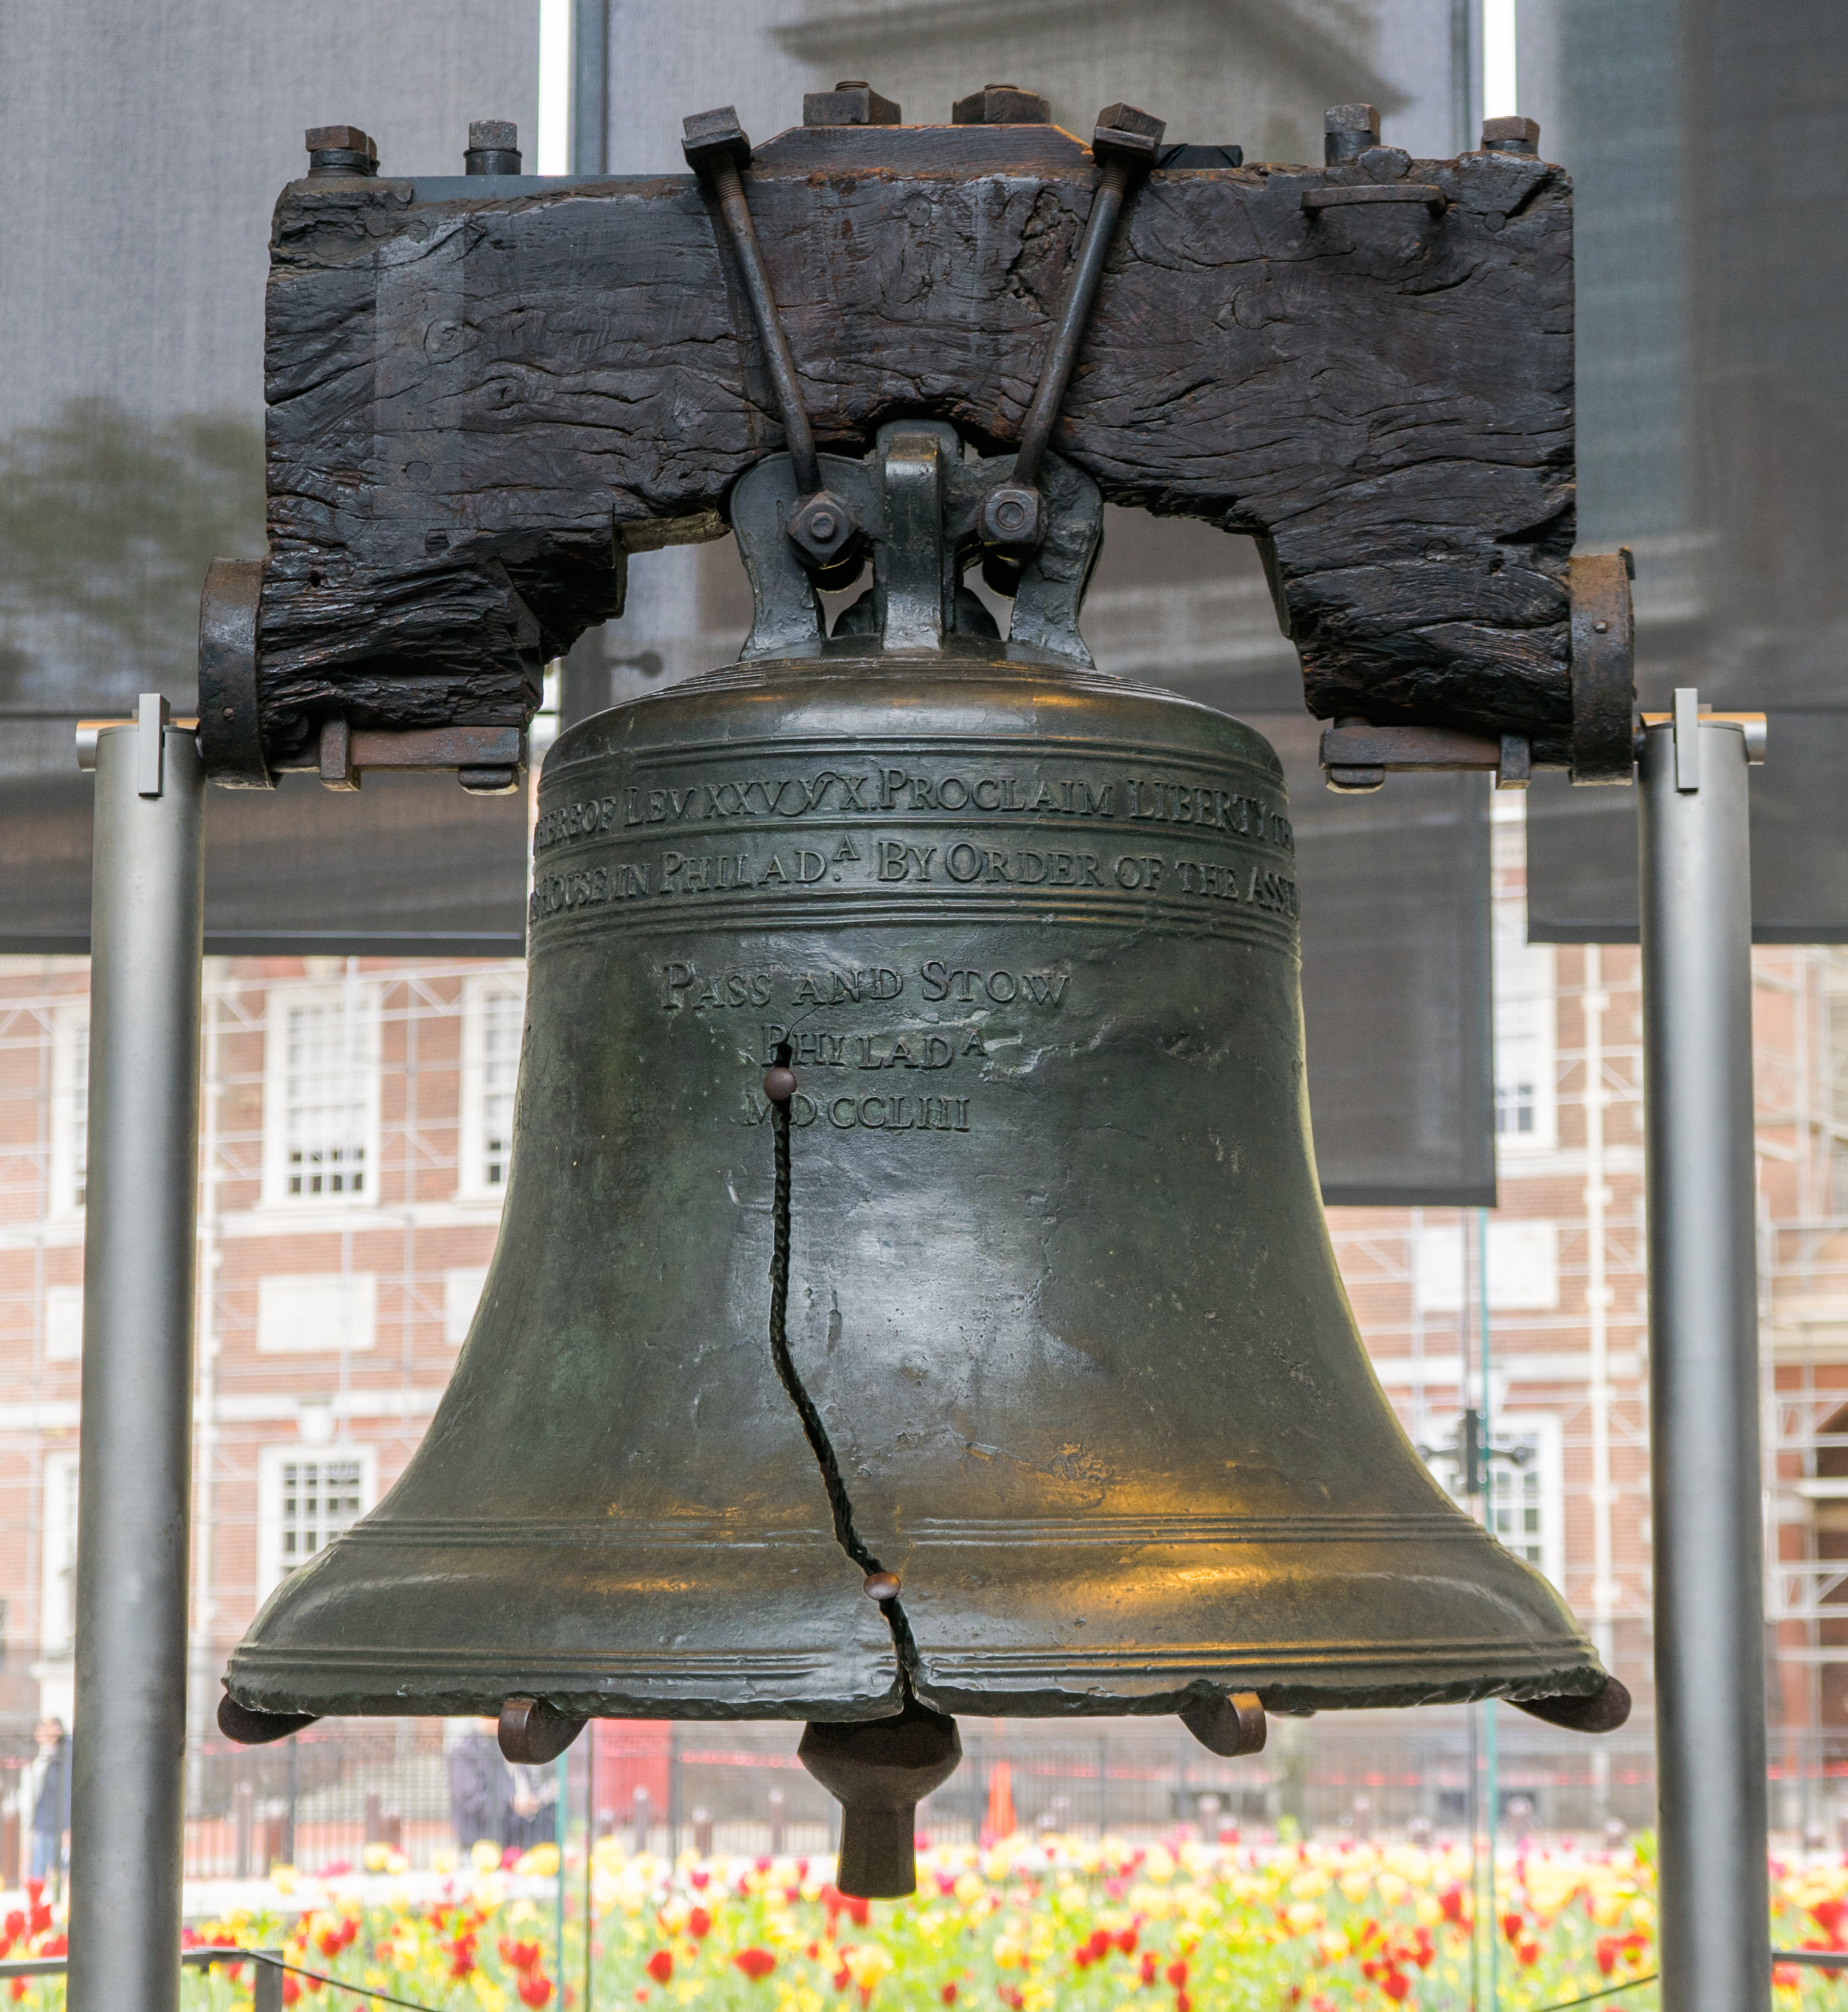
\includegraphics[width=0.3\linewidth]{LibertyBell}
\caption{Liberty Bell}
\label{bell}
\end{figure}

\subsubsection{King George III} \label{george3}
King George III (1738-1820) was the grandson of George 
II. He only learned to read at the age of eleven. In 1760 
he became king, and the next year married Charlotte 
of Mecklenburg-Strelitz, a German princess, who would 
bear him 15 children. He was a devoted family man, 
enjoyed gardening, and was a voluminous reader. His 
royal collection of 65,000 books was given to the British 
Museum. Although his reign did not end until his death 
in 1820, mental instability, diagnosed today as hereditary 
porphyria, effectively ended it in 1811, at which point 
his son, later George IV, became prince regent.

\subsection{Thomas Jefferson}
The Virginian Thomas Jefferson, born April 13, 1743, was 
not a brilliant orator, yet he is the acknowledged author of 
the Declaration of Independence. An accomplished scholar, 
he spoke five languages, was a gifted writer, inventor, 
philosopher, and naturalist, and assembled a collection 
of books that became the embryonic Library of Congress. 
During the revolution, and later as the Constitution was 
being debated, he served the country as an ambassador in 
France, and served as the nation’s third president from 1801 
to 1809.

\section{The Constitution}
The United States Constitution is America’s instruction book. A faded, barely legible set of parchment 
pages, the original signed document was handwritten in iron gall ink with a feathered quill pen. Cast in 
eighteenth-century language and preserved in archival security, it is now available for public view and 
contemplation. The Constitution’s present-day fragile appearance, however, masks the muscle and power of its 
carefully chosen words; forged at a time when life, death, and government rested in the ruling doctrine of divine 
right of kings.

\begin{figure}[h]
\centering
\includegraphics[width=0.3\linewidth]{UnitedStatesDeclarationofIndependence}
\caption{United States Declaration of Independence}
\end{figure}


\end{document}